We have established that there are pronounced gender differences in the patterns of positive and statistically significant treatment effects.\footnote{We summarize previous research on gender differences in Table~\ref{tab:litreview-table}.} Figure~\ref{fig:ppositive} reports the estimated combining functions by gender by category of care used by the control group. When we divide the sample by gender and take-up of alternative formal childcare, samples are small and differences are less precisely determined.\footnote{See Appendix~\ref{appendix:results} for estimates of individual treatment effects and additional specifications of combining functions.}

The null hypothesis  of no treatment effect is equivalent to the hypothesis that the proportion of outcomes is equal to $0.500$. Figure~\ref{fig:ppositivehome} displays combining functions for treatment effects comparing treatment outcomes for ABC/CARE to outcomes for those who stay at home. Figure~\ref{fig:ppositivealternative} displays comparable combining functions comparing treatment effects for outcomes for participating in ABC/CARE to outcomes for those who attend alternative formal childcare. Both of these estimates account for selection into the mode of childcare using matching.

Comparing ABC/CARE to those who stay at home (Figure~\ref{fig:ppositivehome}), a higher proportion of the treatment effects are positive for women than for men. While the female proportion is statistically significantly larger than $0.500$, the male proportion is not. Figure~\ref{fig:ppositivealternative} shows a different pattern comparing ABC/CARE to those who attended alternative formal childcare. Close to 75\% of the treatment effects are positive for men. For women, the proportion of positive treatment effects is similar to the proportion obtained by comparing ABC/CARE to those who stay at home. From this analysis, we conclude that ABC/CARE was effective for men compared to alternative formal childcare programs, but not when compared to staying at home. ABC/CARE was effective for women regardless of the mode of childcare used by the controls.\footnote{Disaggregating by outcome, gender, and mode of childcare for controls produces a noisy pattern that is broadly consistent in Figure~\ref{fig:ppositive}.}

\begin{figure}[!htbp]
\centering
\caption{Positively Impacted Outcomes, ABC/CARE Males and Females}\label{fig:ppositive}
\begin{subfigure}[h]{0.5\textwidth}
		\centering
		\caption{ Treatment vs.\ Stay at Home} \label{fig:ppositivehome}
		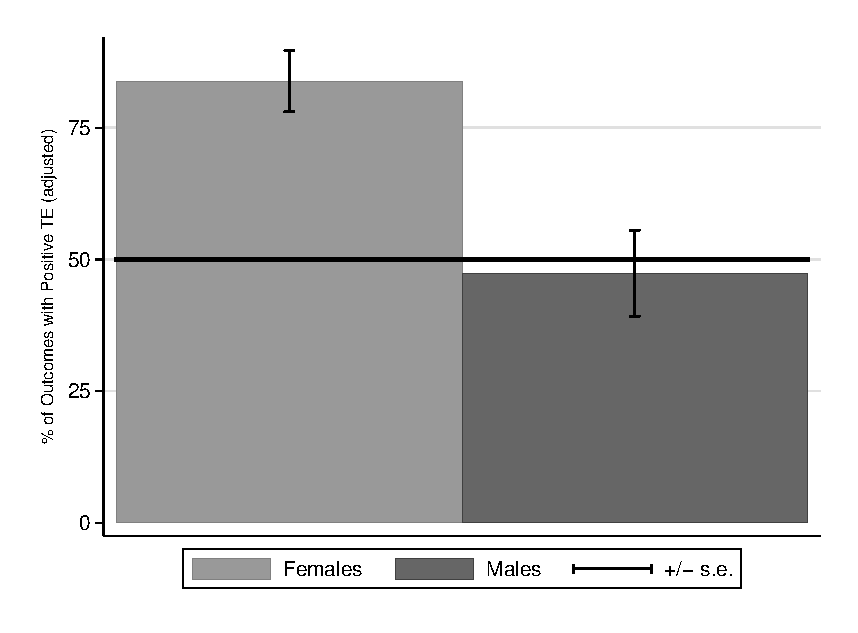
\includegraphics[width=\textwidth]{output/epan_ipw_p0_all.eps}
\end{subfigure}%
\begin{subfigure}[h]{0.5\textwidth}
	\centering
	\caption{Treatment vs.\ Alternative Formal Childcare} \label{fig:ppositivealternative}
		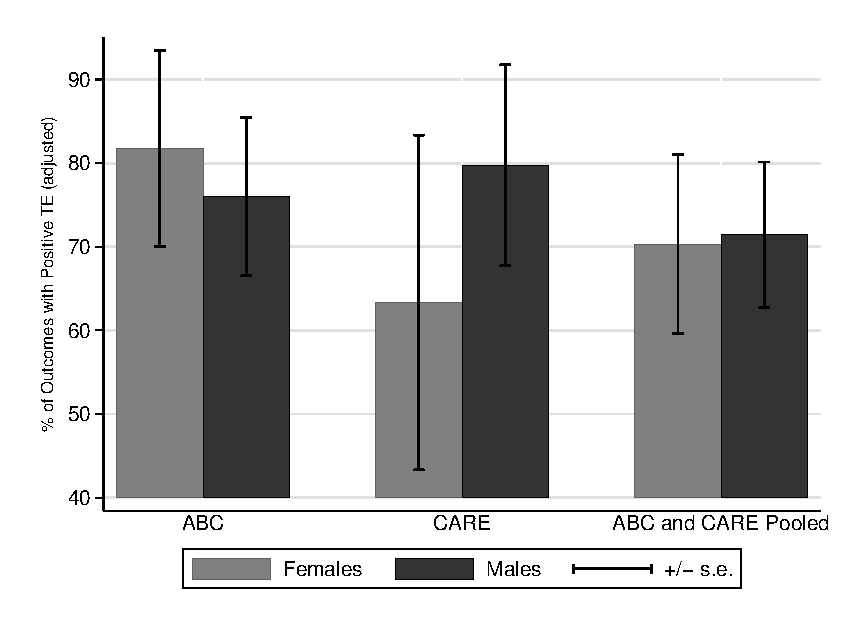
\includegraphics[width=\textwidth]{output/epan_ipw_p1_all.eps}
\end{subfigure}
\footnotesize \justify
\textbf{Note:} Panel (a) displays the percentage of positive treatment effects in accordance with the parameter in Equation~\eqref{eq:cont1}---treatment vs. staying at home---by gender. Panel (b) is analogous for Equation~\eqref{eq:cont2}---treatment vs.\ alternative formal childcare. Standard errors are based on the empirical bootstrap distribution. The null hypothesis is that the proportions of positive treatment effects are greater than 50\%. For a full list of the estimated combining functions, see Appendix~\ref{appendix:results}. \\
\end{figure}

\begin{sidewaysfigure}[!htpb]
\centering
\caption{Gender and Baseline Socioeconomic Disadvantage in the Control Group} \label{figure:socdis}
\begin{subfigure}[h]{0.4\textwidth}
	\centering
	\caption{Take-up of Alternatives by Gender} \label{figure:altgender}
	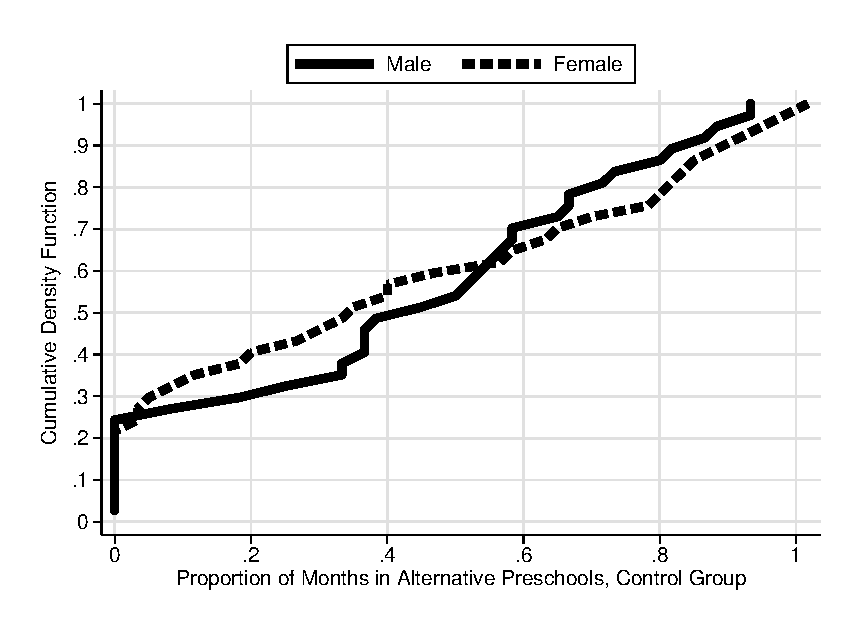
\includegraphics[width=\textwidth]{output/abccare_controlcontamination_boysgirls}
\end{subfigure}%
\begin{subfigure}[h]{0.4\textwidth}
	\centering
	\caption{Socioeconomic Disadvantage by Gender} \label{figure:disadgender}
	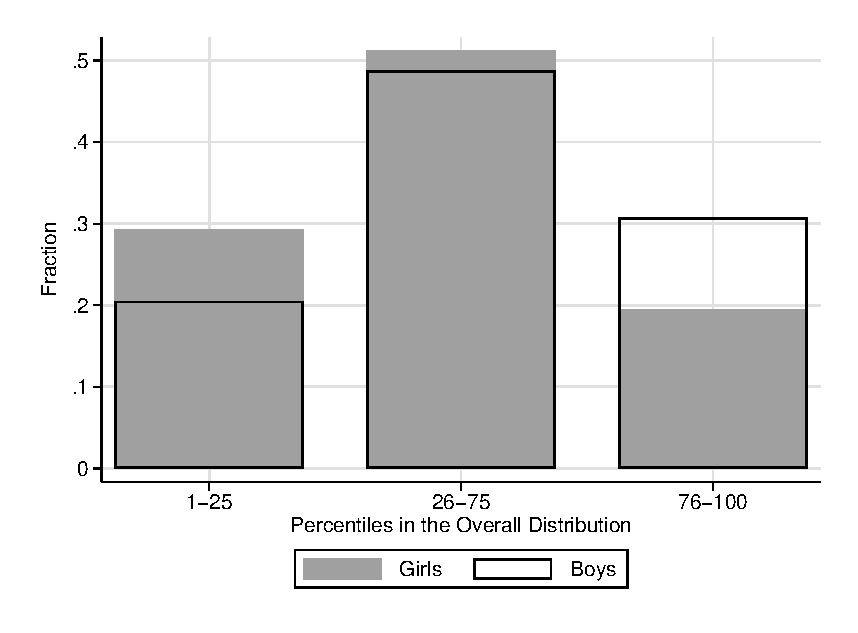
\includegraphics[width=\textwidth]{output/factorbase_girlsboyscompare}
\end{subfigure}
\begin{subfigure}[h]{0.4\textwidth}
	\centering
	\caption{Disadvantage by Take-up of Alternatives, Girls} \label{figure:disadgirls}
	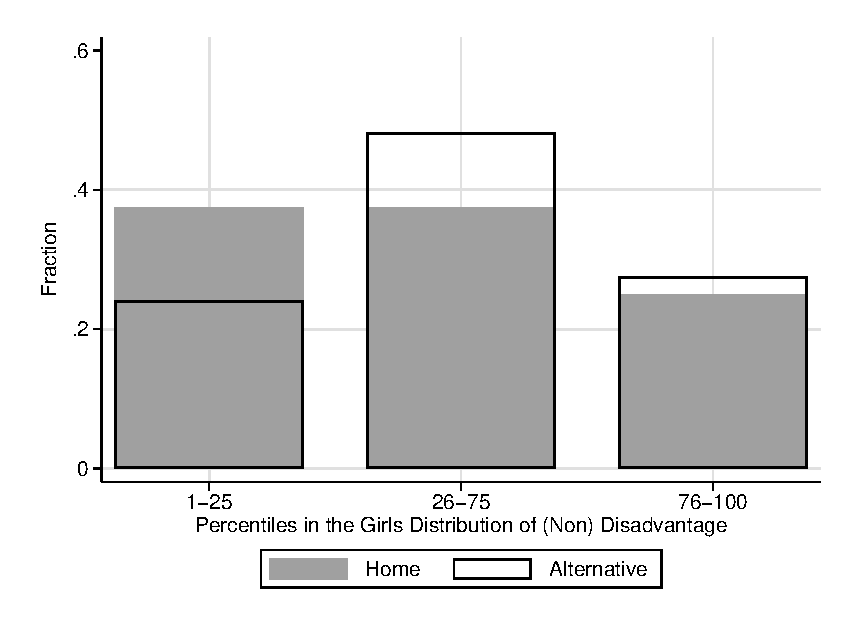
\includegraphics[width=\textwidth]{output/factorbase_wgirlscompare}
\end{subfigure}%
\begin{subfigure}[h]{0.4\textwidth}
	\centering
	\caption{Disadvantage by Take-up of Alternatives, Boys} \label{figure:disadboys}
	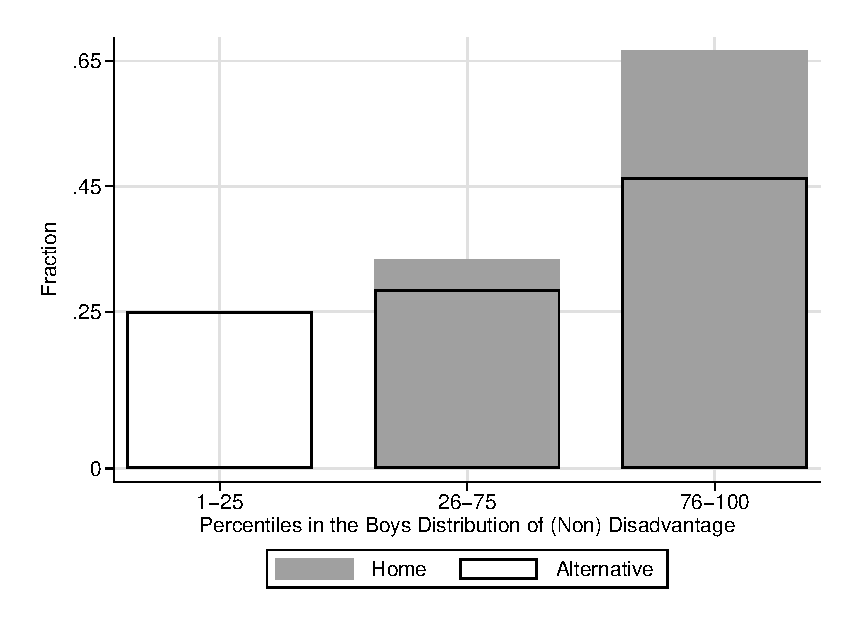
\includegraphics[width=\textwidth]{output/factorbase_wboyscompare}
\end{subfigure}
\footnotesize
\justify
\textbf{Note:} Panel (a) displays the cumulative distribution function of enrollment in alternatives by gender. Panel (b) displays how girls and boys separately fit into the overall (girls and boys pooled) distribution of socioeconomic disadvantage. Panel (c) displays how girls who did not enroll and girls who enrolled in alternatives fit into the overall female distribution of socioeconomic disadvantage. Panel (d) is analogous to Panel (c) for boys. Our measure of socioeconomic disadvantage is a latent of the following variables: Maternal age, education, and IQ, as well as number of siblings and HRI score.
\end{sidewaysfigure}

This difference suggests that boys and girls faced different situations in their control group condition, especially in their home environments.\footnote{Table~\ref{table:controlsubscharacteristics} summarizes the baseline characteristics by gender and mode of childcare.} About the same percentage of control-group girls attended alternative formal childcare (73\%) as did control-group boys (76\%). See Figure~\ref{figure:altgender}. No girls who stayed at home had working mothers at baseline while 23\% of the girls who attended alternative formal childcare had mothers working at baseline. For boys, 14\% of those who stayed at home had mothers working at baseline while 29\% of those who attended alternative formal childcares had working mothers.

As shown in Section~\ref{sec:treatment-effects}, the childcare supplied by ABC/CARE increases maternal employment and family income in childhood. This effect is especially pronounced for girls. Differentially higher employment of mothers leads to higher income for families of girls as a result of the childcare afforded mothers. HOME scores are differentially enhanced for girls.

More fathers are present for boys. At baseline, this leads to higher family income for boys. However, the program does not attract absent fathers to come home. Family income is higher for boys than girls after treatment is administered, but this is true for both treatment and control boys compared to girls. Boys appear to benefit from the greater presence of the father, but there is no program-induced treatment effect on inducing fathers into the home.

To formally test the differences in home-life advantage between control-group girls and boys, we create an index of socioeconomic disadvantage at baseline using the following variables: Mother's age, education, IQ, marital status, and employment, as well as number of children and father's presence at home. This index is distinct from HRI. We assess how girls and boys fit into the overall distribution of this latent measure in the control group. Boys are disproportionately more advantaged than girls (Panel~\ref{figure:disadgender}).

Because girls' families were more resource-constrained compared to their male counterparts, girls in the control group were raised in a more disadvantaged environment or went to lower-quality preschools. Thus, as documented in Section~\ref{sec:treatment-effects}, they benefited more from ABC/CARE than boys when compared to the next best alternative as perceived by their parents,.

Table~\ref{table:disadtests} uses our constructed measure of disadvantage to test the difference in baseline disadvantage across boys and girls. We reject the null of a common distribution of our measure of socioeconomic disadvantage across girls and boys (at baseline). In Panels~\ref{figure:disadgirls} and~\ref{figure:disadboys} of Figure~\ref{figure:socdis}, we further dissect socioeconomic disadvantage within genders, and provide the corresponding tests in Table~\ref{table:disadtests}. \textbf{[JJH: I keep asking for the index post-baseline including the wife's income induced by program.] [JLG: We cannot form the index post-baseline. This morning you said that this was ``unfortunate'' but we seemed to understand that was a fact. We have parental income and we have HOME scores (parenting) and both are included in Tables 1 and 4.] [JJH: It is not a ``fact'' --- it is your unwillingness to report age 12 results.] [JLG: No. Please don't take it that way. I prepared a table with these results and answers to your last e-mail in the memo that I sent today. - June 14 memo.]}

\begin{table}[!htpb]
\begin{threeparttable}
\caption{Gender and Baseline Socioeconomic Disadvantage in the Control Group} \label{table:disadtests}
\centering
\begin{tabularx}{16.5cm}{XcX}
& \begin{tabular}{ccccc}
\toprule
& Males vs. Females & & \mc{2}{c}{Alternatives vs. Home} \\
& & & Males & Females \\
\midrule
 \citet{Rosenbaum_2005_Distribution_JRSS}  & \\
$p$-value & \textbf{0.007} & & \textbf{0.006} & 0.110 \\
\bottomrule
\end{tabular}


% Control, males vs. females: distance between: factor of m_age_base, m_ed_base, m_iq_base, hh_sibs_base, hrabc_index

% Alt. vs home: factor of m_age_base, m_ed_base, m_iq_base, hh_sibs_base, hrabc_index &
\end{tabularx}
\begin{tablenotes}
\footnotesize
\item \textbf{Note:} Row [1] displays an exact, non-parametric $p$-value for the null hypothesis that the control males and control females have the same level of disadvantage. Row [2] displays the same $p$-value for the null  hypothesis that within males, those who attend alternative formal childcare and those who stay at home have the same level of disadvantage. Row [3] is analogous to Row [2] except for females. These tests all use a latent measure of socioeconomic disadvantage (mother's age, education, IQ, marital status, and employment, as well as number of siblings and father's presence at home). Under the null hypotheses, the pairs with the closest distance in disadvantage would be comprised of one male and one female (for the comparison of males vs. females). Rejecting the null implies that the distributions are significantly different. Statistics significant at the $0.10$ level are bolded.
\end{tablenotes}
\end{threeparttable}
\textbf{[JJH: Can we do same test, say at post-baseline age 5? Later? I am asking for one post-baseline income.] [JLG: Ideally, we would have a time series of the measure of disadvantage for each child. I think we both agree on that. But we don't have that. A time series of the home score, for which we do have results, is in the paper both in Table 1 (the analogous test of Table 5 is in there) and Table 4, which are by gender and comparing boys and girls. We call this ``parenting'' in the paper. The measure of parental income used in the paper is an aggregate of mother's, father's, or both mother's and father's incomes. The reason for using the different variables is that at different ages we observe different measures of income. We also present treatment effects of this by gender in Tables 1 and 4.] [JJH: We have a measure of father's income at age 4 or so you said earlier -- we do not know family income at age 5? We want] [JLG: See the previous answer and also I said father's income is at ages 12 and 21. But we do have and display what we have, which is explained above, at from ages 1 to 5.] [JJH: Jorge, can I read and I read that it was 12 and I asked if there is a treatment effect that differs by gender.] [JLG: Please see the memo for that. We report the treatment effects by gender.]
}
\end{table}

Parents of more advantaged girls are more likely to send their daughters to alternative preschools. Parents of more advantaged boys are more likely to keep their sons at home. Thus, boys benefited more from treatment when compared to attending alternative formal childcare as opposed to staying at home where they faced better environments than girls. The opposite pattern holds for girls, although the differences between the estimates by counterfactual scenario are smaller for girls than for boys. \textbf{[JJH: I need post-baseline, say age income.] [JLG: The measure of parental income in Tables 1 and 4 contains: measures of mother labor supply and mother's income between ages 1 and 5. The father's income (ages 12 and 21) would bring the observations to a very low level. That's as far as we can go without getting a very low number of observations.] [JJH: Something is better than nothing --- what is ``low'' and what is ``high'' --- please what is it?] [JLG: Please see Table 2 in the June, 14 memo. We reported there the number of observations.]
[JLG: Also, this is post-treatment. Note that the results regarding this variables in both Tables 1 and 4 is consistent with the rest of the story: females benefit more than males and post-treatment gaps are reduced.]}

Table~\ref{table:disadtests} confirms this point. It shows that selection into alternative formal childcare statistically significantly differs by family disadvantage for boys, while it is not statistically significant for girls.

